\section{Honey Encryption - Ein Beispiel}

\begin{frame}[c]
	\frametitle{Honey Encryption - Ein Beispiel}
	
	\begin{figure}
	\center
	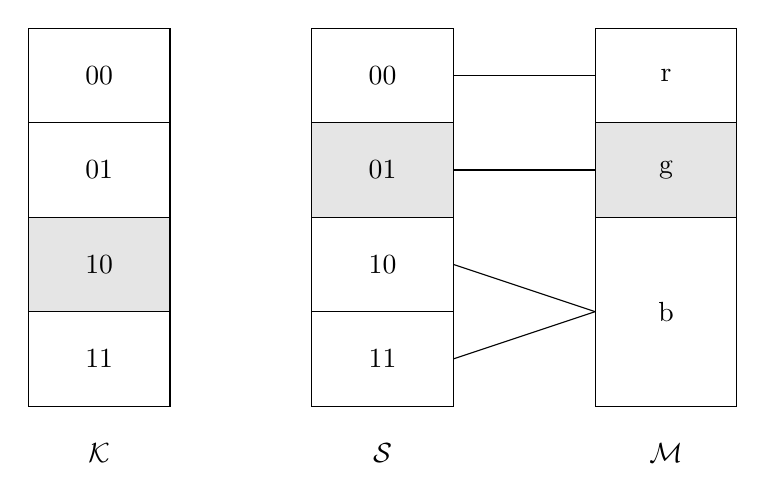
\begin{tikzpicture}[scale=0.6]
		% Linker Kasten
		\draw (1, 8) rectangle ++ (3, 2) node [midway] {$00$};
		\draw (1, 6) rectangle ++ (3, 2) node [midway] {$01$};
		\draw [fill=lightgray!40!white] (1, 4) rectangle ++ (3, 2) node [midway] {$10$};
		\draw (1, 2) rectangle ++ (3, 2) node [midway] {$11$};
		% Mittlerer Kasten
		\draw (7, 8) rectangle ++ (3, 2) node [midway] {$00$};
		\draw [fill=lightgray!40!white] (7, 6) rectangle ++ (3, 2) node [midway] {$01$};
		\draw (7, 4) rectangle ++ (3, 2) node [midway] {$10$};
		\draw (7, 2) rectangle ++ (3, 2) node [midway] {$11$};
		% Rechter Kasten
		\draw (13, 8) rectangle ++ (3, 2) node [midway] {r};
		\draw [fill=lightgray!40!white] (13, 6) rectangle ++ (3, 2) node [midway] {g};
		\draw (13, 2) rectangle ++ (3, 4) node [midway] {b};
		% Labels unten
		\node at (2.5, 1) {$\mathcal{K}$};
		\node at (8.5, 1) {$\mathcal{S}$};
		\node at (14.5, 1) {$\mathcal{M}$};
		% Linien
		\draw (10, 9) --++ (3, 0);
		\draw (10, 7) --++ (3, 0);
		\draw (10, 5) --++ (3, -1);
		\draw (10, 3) --++ (3, 1);
	\end{tikzpicture}
	\end{figure}
\end{frame}



\begin{frame}[t]
	\frametitle{Honey Encryption - Ein Beispiel}

	\begin{columns}
	
	\column{0.5\textwidth}

		\begin{figure}
		\center
		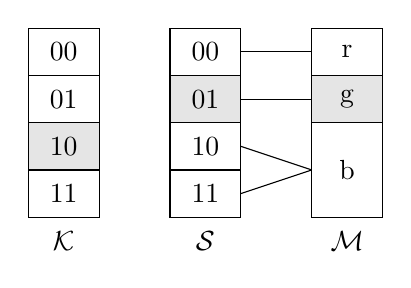
\begin{tikzpicture}[scale=0.3]
			% Linker Kasten
			\draw (1, 8) rectangle ++ (3, 2) node [midway] {$00$};
			\draw (1, 6) rectangle ++ (3, 2) node [midway] {$01$};
			\draw [fill=lightgray!40!white] (1, 4) rectangle ++ (3, 2) node [midway] {$10$};
			\draw (1, 2) rectangle ++ (3, 2) node [midway] {$11$};
			% Mittlerer Kasten
			\draw (7, 8) rectangle ++ (3, 2) node [midway] {$00$};
			\draw [fill=lightgray!40!white] (7, 6) rectangle ++ (3, 2) node [midway] {$01$};
			\draw (7, 4) rectangle ++ (3, 2) node [midway] {$10$};
			\draw (7, 2) rectangle ++ (3, 2) node [midway] {$11$};
			% Rechter Kasten
			\draw (13, 8) rectangle ++ (3, 2) node [midway] {r};
			\draw [fill=lightgray!40!white] (13, 6) rectangle ++ (3, 2) node [midway] {g};
			\draw (13, 2) rectangle ++ (3, 4) node [midway] {b};
			% Labels unten
			\node at (2.5, 1) {$\mathcal{K}$};
			\node at (8.5, 1) {$\mathcal{S}$};
			\node at (14.5, 1) {$\mathcal{M}$};
			% Linien
			\draw (10, 9) --++ (3, 0);
			\draw (10, 7) --++ (3, 0);
			\draw (10, 5) --++ (3, -1);
			\draw (10, 3) --++ (3, 1);
		\end{tikzpicture}
		\end{figure}

	\vspace*{0.5cm}

	\pause
	
	Verschlüsselung
	\begin{align*}
	&01  \leftarrow \text{Nachricht } M \textit{ (grün)} \\
	\oplus&\underline{10}  \leftarrow \text{Schlüssel }K\\
	&11  \leftarrow \text{Ciphertext }C
	\end{align*}
	
	\pause

	\column{0.5\textwidth}

	Entschlüsselung
	\begin{align*}
	&11 \leftarrow \text{Ciphertext }C\\ 
	\oplus&\underline{10} \leftarrow\text{Schlüssel }K\\
	&01 \leftarrow\text{Nachricht } M \textit{ (grün)} 
	\end{align*}

	\pause

	Brute-Force-Angriff
	\begin{align*}
	&11 \leftarrow \text{Ciphertext }C\\ 
	\oplus&\underline{11} \leftarrow\text{Schlüssel }K'\\
	&00 \leftarrow\text{Nachricht } M' \textit{ (rot)} 
	\end{align*}

	\end{columns}
\end{frame}